\paragraph{IUP02.1 Modificar contraseña} \hspace{1cm}\\ 
\label{pant:IUP02.1}

\textbf{\textcolor[rgb]{0, 0, 0.545098} {Objetivo}}\\
Esta pantalla permite al Practicante modificar su contraseña actual.\\

\textbf{\textcolor[rgb]{0, 0, 0.545098}{Diseño}}\\
La figura \ref{fig:IUP02.1} muestra al Practicante los campos requeridos para modificar su contraseña. \\

En la parte inferior derecha se encuentran los botones Guardar y Cancelar, los cuales corresponden a modificar su contraseña actual o cancelar la operación, respectivamente.\\

\begin{figure}[H]
	\centering
		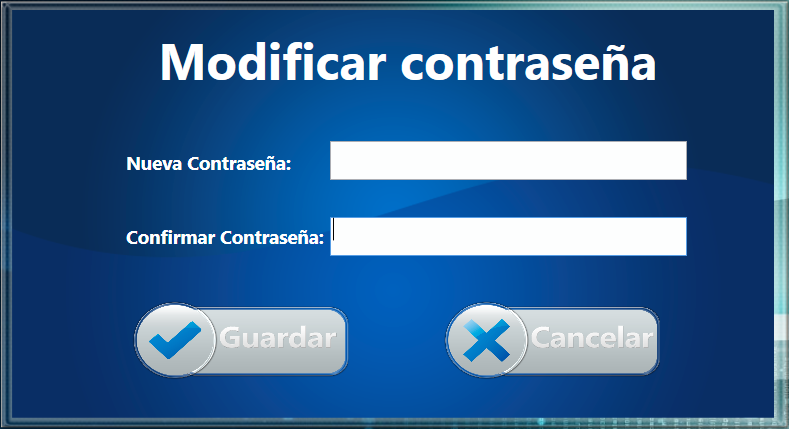
\includegraphics[scale=0.8]{./Figuras/Pantallas/IUP02_1Modificar_contrasena}
	\caption{IUP02.1 Modificar contraseña}
	\label{fig:IUP02.1}
\end{figure}

\textbf{\textcolor[rgb]{0, 0, 0.545098}{Entradas}}\\
En esta pantalla el Practicante debe capturar la siguiente información:

\begin{itemize}
	\item La Nueva contraseña.
	\item La Confirmación de la contraseña.
\end{itemize}

\textbf{\textcolor[rgb]{0, 0, 0.545098}{Comandos}}	
\begin{itemize}
	\item \textbf{\textcolor[rgb]{0, 0, 0.545098}{Guardar:}} Permite al Practicante registrar la nueva contraseña cuando la información ingresada en los campos obligatorios sea correcta.
	\item \textbf{\textcolor[rgb]{0, 0, 0.545098}{Cancelar:}} Descarta la información registrada y muestra la pantalla \nameref{pant:IUP02}.
\end{itemize}
\vspace{1em}

\textbf{\textcolor[rgb]{0, 0, 0.545098}{Mensajes}}\\

\textbf{\nameref{msj:MSG01}}: Se muestra en la pantalla \nameref{pant:IUP02.1} indicando que la herramienta ha actualizado la contraseña de manera exitosa.\\

\textbf{\nameref{msj:MSG12}}: Se muestra en la pantalla \nameref{pant:IUP02.1} cuando el Practicante no haya ingresado campos obligatorios.\\

\textbf{\nameref{msj:MSG13}}: Se muestra en pantalla cuando el Practicante haya ingresado datos con un formato incorrecto en algún campo.\\

\textbf{\nameref{msj:MSG14}}: Se mostrará en pantalla cuando el Practicante haya ingresado contraseñas que no coinciden en ambos campos.\\

\clearpage